\documentclass[aspectratio=169]{beamer}

\usepackage{tikzlings}

\setbeamertemplate{navigation symbols}{}

% trick taken from https://topanswers.xyz/tex?q=1989
\tikzset{
    use page relative coordinates/.style={
        shift={(current page.south west)},
        x={(current page.south east)},
        y={(current page.north west)}
    },
}

\usepackage{xfp}
\ExplSyntaxOn
\let\intmodnn\int_mod:nn
\ExplSyntaxOff


\begin{document}
	
\begin{frame}
  \begin{tikzpicture}[remember picture, overlay,use page relative coordinates]
    \node at (0.5,0.6) {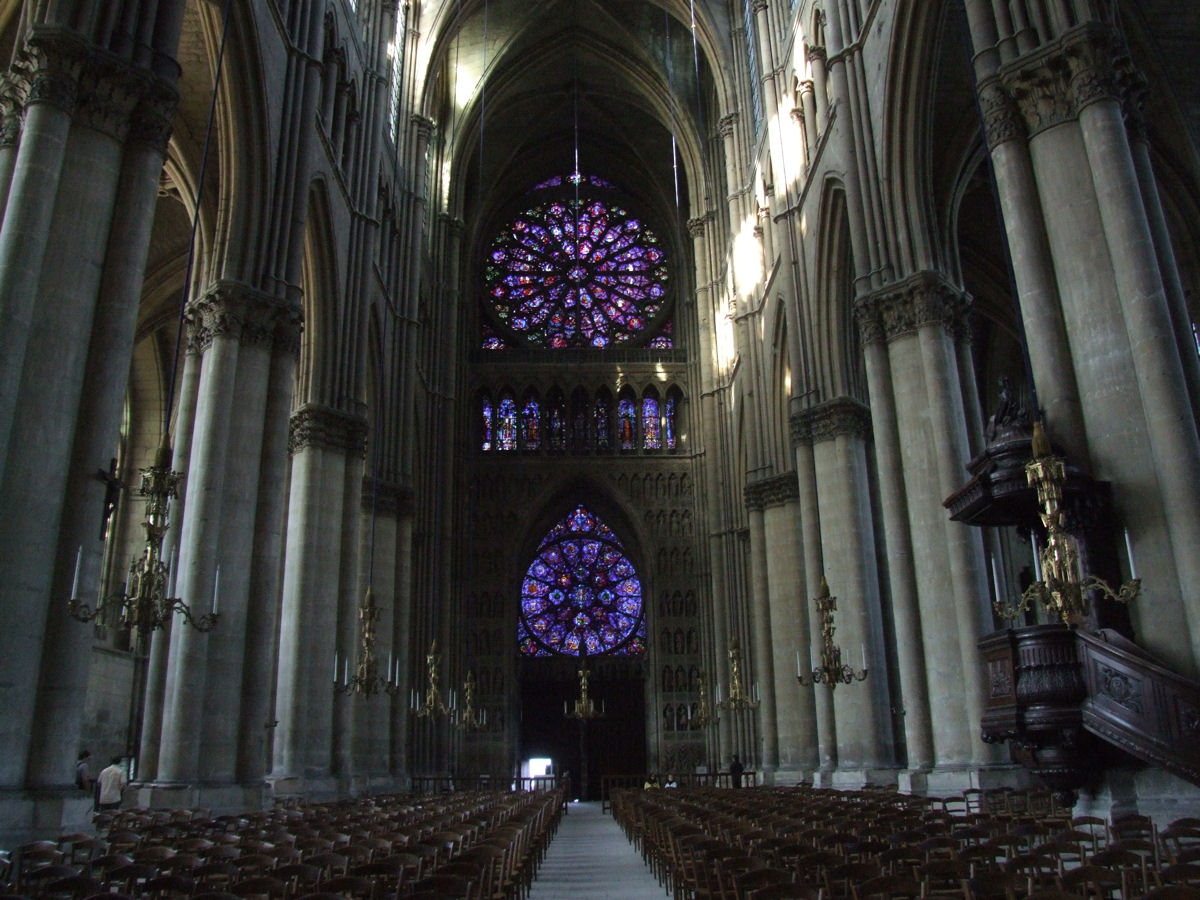
\includegraphics[width=\paperwidth]{./include/Reims_Cathedrale_Notre_Dame_interior_001}};
		\node[xscale=1.2] at (0.48,0.86) {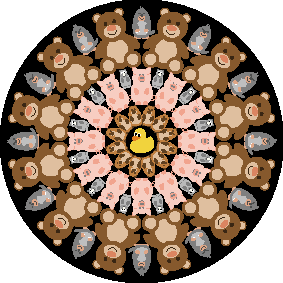
\includegraphics[width=2cm]{./include/mandala}};
		\node[xscale=1.03] at (0.485,0.381) {
\includegraphics[width=1.55cm]{./include/mandala2}};    
    
    \ifnum \intmodnn{\thepage}{20} > 10
      \def\pandastate{panda1}
    \else
      \def\pandastate{panda2}
    \fi
    
    \node[anchor=south,rotate=10*cos(5*\thepage)] at (0.15,0.03) {\includegraphics[width=1cm]{./include/\pandastate}};
    \node[anchor=south,rotate=10*cos(5*\thepage)] at (0.25,0.05) {\includegraphics[width=1cm]{./include/\pandastate}};
    \node[anchor=south,rotate=10*cos(5*\thepage)] at (0.35,0.03) {\includegraphics[width=1cm]{./include/\pandastate}};
    \node[anchor=south,rotate=10*cos(5*\thepage)] at (0.45,0.05) {\includegraphics[width=1cm]{./include/\pandastate}};
    \node[anchor=south,rotate=10*cos(5*\thepage)] at (0.55,0.03) {\includegraphics[width=1cm]{./include/\pandastate}};
    \node[anchor=south,rotate=10*cos(5*\thepage)] at (0.65,0.05) {\includegraphics[width=1cm]{./include/\pandastate}};
    \node[anchor=south,rotate=10*cos(5*\thepage)] at (0.75,0.03) {\includegraphics[width=1cm]{./include/\pandastate}};
    \node[anchor=south,rotate=10*cos(5*\thepage)] at (0.85,0.05) {\includegraphics[width=1cm]{./include/\pandastate}};            

    % credit for background image
    \node[white,text width=.8\paperwidth,font=\tiny,align=center] at ([yshift=0.35cm]current page.south) {Image source: \url{https://upload.wikimedia.org/wikipedia/commons/f/fb/Reims_Cathedrale_Notre_Dame_interior_001.JPG}};  
    
  \end{tikzpicture}
  \pause[600]
\end{frame}	
	
\end{document}